\section{Preliminaries}
\label{sec:background}
\newcommand{\satisfies}{\vdash_{\!\!s}}
\newcommand{\nsatisfies}{\nvdash_{\!\!s}}
\newcommand{\bool}[0]{\mathit{bool}}
\newcommand{\reach}[0]{\mathit{R}}
\newcommand{\ite}[3]{\mathit{if}\ {#1}\ \mathit{then}\ {#2}\ \mathit{else}\ {#3}}


\subsection{Models, Requirements, and Provability}

Given a state space $U$, a transition system $(I,T)$ consists of an
initial state predicate $I : U \to \bool$ and a transition step
predicate $T : U \times U \to \bool$. We define the notion of
reachability for $(I, T)$ as the smallest predicate $\reach : U \to
\bool$ which satisfies the following formulas:
\begin{gather*}
  \forall s.~ I(u) \Rightarrow \reach(u) \\
  \forall u, u'.~ \reach(u) \land T(u, u') \Rightarrow \reach(u')
\end{gather*}
A safety property $P : U \to \bool$ is a state predicate that holds on a transition system $(I, T)$ if it holds on all
reachable states, i.e., $\forall u.~ \reach(u) \Rightarrow P(u)$,
written as $\reach \Rightarrow P$ for short. When this is the case, we
write $(I, T)\vdash P$. To generalize the notion of transition system, especially in SMT-based model checking, it is assumed that the transition relation has the structure of a top-level conjunction. This assumption gives us a structure that we can easily manipulate. Given $T(u, u') = T_1(u, u') \land \cdots \land T_n(u, u')$ we will write $T = T_1 \land \cdots \land T_n$ for short.
By further abuse of notation,
$T$ is identified with the set of its top-level conjuncts. Thus, $x \in
T$ means that $x$ is a top-level conjunct of $T$, and $S
\subseteq T$ means all top-level conjuncts of $S$ are top-level
conjuncts of $T$. When a top-level conjunct $x$ is removed from $T$, it is written as $T \setminus \{x\}$. Such a transition system can easily encode our example model in Section~\ref{sec:example}.  We assume each equation defines a conjunct within the transition system which we will denote by the variable assigned, so $T = \{$ {\small \texttt{a1\_below, a2\_below, a1\_above, a2\_above, below, above\_hyst}} $\}$.


\begin{definition}{\emph{Inductive Validity Core:}}
  \label{def:ivc}
  Given $(I, T)\vdash P$, $S \subseteq
  T$ is an {\em Inductive Validity Core} for $P$
  \emph{iff} $(I, S) \vdash P$.
\end{definition}

In examining provability, we are interested in {\em minimal} sets that satisfy a property $P$; tracing a property to the entire model is not particularly enlightening.

\begin{definition}{\emph{Minimal Inductive Validity Core (IVC):}}
  \label{def:minimal-ivc}
  Inductive validity core $S$ for $(I, T)\vdash P$ is minimal, denoted $IVC(P, S)$, iff
  $\neg\exists S' \subset S .\quad (I, S') \vdash P $.
\end{definition}

\begin{note}{}
Hereafter, the term ``IVC'' refers to a \textbf{minimal} IVC.
\end{note}

Note that there could be many IVCs for a given property, corresponding to different proofs. To capture that notion, we define \emph{all IVCs ($AIVC$)} for a property as an association to all its IVCs.

$$ AIVC(P) \equiv  \{\ S~|~S \subseteq T \land  IVC(P, S)\} $$

%In the example in Fig. \ref{fig:asw}, as visualized in part (b),
%$AIVC ({\tt P}) = \{\{{\tt P}, {\tt c2}, {\tt c3}\}, \{{\tt P}, {\tt x}, {\tt c3}\}\}$.
\noindent The set of $AIVC$-s for all properties represents the complete traceability of the system. Establishing the $AIVC$ for a single property, one gets a clear picture of the all the model elements that are necessary to prove the property.

\subsection{Coverage and Mutations}
In general, specification completeness can be defined with
regard to the notion of coverage. In fact, the way that coverage
is formalized plays a key part in the strength/ effectiveness of
a method for the assessment of completeness. The goal of a coverage metric is usually to assign a numeric score that describes how well properties cover the design. The majority of the work on coverage metrics has focused on {\em mutations}, which are ``atomic'' changes to the design, where the set of possible mutations depends on the notation that is used.  A mutant is ``killed'' if one of the properties that is satisfied by the original design is violated by the mutated design~\cite{chockler_coverage_2003,chockler2001practical,chockler2010coverage,Kupferman:2006:SCF,kupferman_theory_2008}.  There are many different kinds of mutations that have been proposed, primarily focused on checking sequential bit-level hardware designs.  For these designs, {\em State-based} mutations flip the value of one of the bits in the state.  There are several variations depending on whether the flip is performed on a single state within a Kripke structure~\cite{hoskote1999coverage}, or in the description of the signal in the transition relation of the circuit~\cite{chockler2001practical}.  {\em Logic-based} mutations fix the value of a bit to constant zero or one, and can be used to determine whether properties can find stuck-at faults.  {\em Syntactic} mutations~\cite{chockler_coverage_2003} remove states in a control flow graph representation of hardware.  Similarly, for software, it is possible to apply any of the ``standard'' source code mutation operators used for software testing~\cite{Andrews06:mutation} towards requirements coverage analysis.  Some examples of software mutations are:
\begin{enumerate}
    \item Replace an integer constant C by one of $\{0, 1, -1, C + 1, C - 1\}$,
    \item Replace an arithmetic, relational, logical, bitwise logical, increment/decrement, or arithmetic-assignment operator by another operator from the same class,
    \item Negate the decision in an if or while statement,
    \item Delete a statement.
\end{enumerate}

We assume each element $T_i \in T$ has a set of possible mutations associated with it.  Depending on the modeling formalism used, this may be the value of a gate or signal or an expression within a statement in a program.  We will further assume the existence of a mutation function $f_{m}$ that, given a model element, will return a finite set of mutations for that element.  We can then define the set of mutant models $M$ as follows:
\[
    M = \{ (T \setminus \{T_i\}) \cup \{m\} \ |\ T_i \in T, m \in f_{m}(T_i) \}
\]

\noindent and then define the mutation score for property $P$ in the standard way:

\begin{definition} {\emph{Generalized mutation coverage.} } \\
\[
   \mutcov = \frac{ | \{m~|~ m \in M(T)~\land~m \nvdash P\} |}{|M(T)|}
\]
\end{definition}
Note that without loss of generality, we consider a single property P, which can be viewed as the conjunction of all the properties of the model.
%\footnote{Besides, the notions provided in this paper can be easily applied to a set of properties.}.

In our example in Figure~\ref{fig:asw}, applying the software mutations from~\cite{Andrews06:mutation} would involve manipulating the constants used in the definitions of \texttt{a1\_below, a2\_below, a1\_above, a2\_above}, swapping 'or' and 'and' in the definition of \texttt{below, above\_hyst}, or negating the conditions in the if/then/else statements.  Even for this small model, there are many possible mutations (57).  The number of single-mutation programs is roughly the product of the leaf elements of the program AST and the size of the chosen set of mutations, which can lead to an impractical number of verification problems.

\newcommand{\andnode}{{\sc and}}
\newcommand{\invnode}{{\sc inv}}
\newcommand{\inpnode}{{\sc inp}}
\newcommand{\regnode}{{\sc reg}}
\newcommand{\mutnode}{{\sc mut}}
\newcommand{\inputnode}{{\sc input}}

Mutations for hardware are discussed in~\cite{chockler2010coverage,Kupferman:2006:SCF,kupferman_theory_2008}.  In most of this work, the hardware model is formalized as an and-inverter-graph net-list, a graph representation of circuits in which vertices are \{\andnode, \invnode\} gates or memory elements (registers) and edges are connections between gates (signals).  Formally, A net-list $N$ is a directed graph $(V_N,E_N, \tau_N)$ where $V_N$ is a finite set of vertices, $E_N \subseteq V_N \times V_N$ is the set of directed edges and $\tau_N : V_N \rightarrow \{$\andnode, \invnode, \regnode, \inpnode$\}$ maps a node to its type, where \andnode\ is an ``and'' gate, \invnode\ is an inverter, \regnode\ is a register, and \inpnode\ is a primary input.  The in-degree of a vertex of type \andnode\ is at least two, of type \invnode\ and \regnode\ is exactly one and of type \inpnode\ is zero. Any cycle in $N$ must contain at least one \regnode\ node~\cite{chockler2010coverage}.

Given this representation, it is possible to discuss mutations of a single vertex: either stuck-at-zero, stuck-at-one, or nondeterministic.  This mutation is performed by changing the vertex to \mutnode, where \mutnode\ can be a ``fresh'' input for non-deterministic mutations, or fixed to 0 or 1 for stuck-at mutations. Formally the semantics of a mutant net-list is defined as a new labeling function:

\[ \tau^{v}_{N}(u) = \begin{cases}
    \tau(v) & \textrm{ if $v \neq u$} \\
    \textrm{\mutnode}   & \textrm{ if $v = u$}
\end{cases}  \]
\noindent

%To mutate a vertex $v_i$, a  multiplexer is added to $N$. Then, the  edges  of  the  net-list are modified such  that  the  tails  of  all  the edges directed from
%$v_i$ are changed to the output of the multiplexer, which replaces
%$E_N$ with a new set of edges $E^{v_i}_M$ in the mutated net-list.
\ela{why don't you bring up the use of multiplexer?}
Let  $N = (V_N,E_N, \tau_N)$ be the original net-list;
when property $P$ satisfied by $N$ fails on the mutant net-list $(V_N, E^{v_i}_N, \tau^{v_i}_{N})$ constructed by a single non-deterministic mutation from $\tau^{v_i}_{N}$, it is said that a mutant is discovered for $P$ (or $v_i$ is covered by $P$). \ela{I think using $\tau^{v}_{N} (v_i)$ it's not correct; I changed it to $\tau^{v_i}_{N}$}
We assume a function $TS : N \rightarrow T$ that returns the corresponding transition system of a net-list.  \ela{shouldn't it be $TS: N \rightarrow I \rightarrow T$ ?}
Given this representation, we can define nondeterministic coverage as follows:

\begin{definition} {\emph{Nondeterministic coverage (\nondetcov) ~\cite{chockler2010coverage}.} }
\label{def:non-det}
Given $N = (V_N,E_N, \tau_N)$,
$v_i \in V_N$ is covered by property $P$ \emph{iff} $v_i \in \nondetcov (P)$, where
$\nondetcov (P) = \{ v_i~|~ v_i \in V_N \wedge TS(N) \vdash P \wedge TS((V_N, E^{v_i}_N, \tau^{v_i}_{N})) \nvdash P \}$.
\end{definition}
Using  $\nondetcov$, the coverage score of specification $P$ is computed by
\[
   \frac{ | \nondetcov (P) |}{|V_N|}
\]


%\fi
%
%\iffalse
%\begin{figure}
%  \centering
%  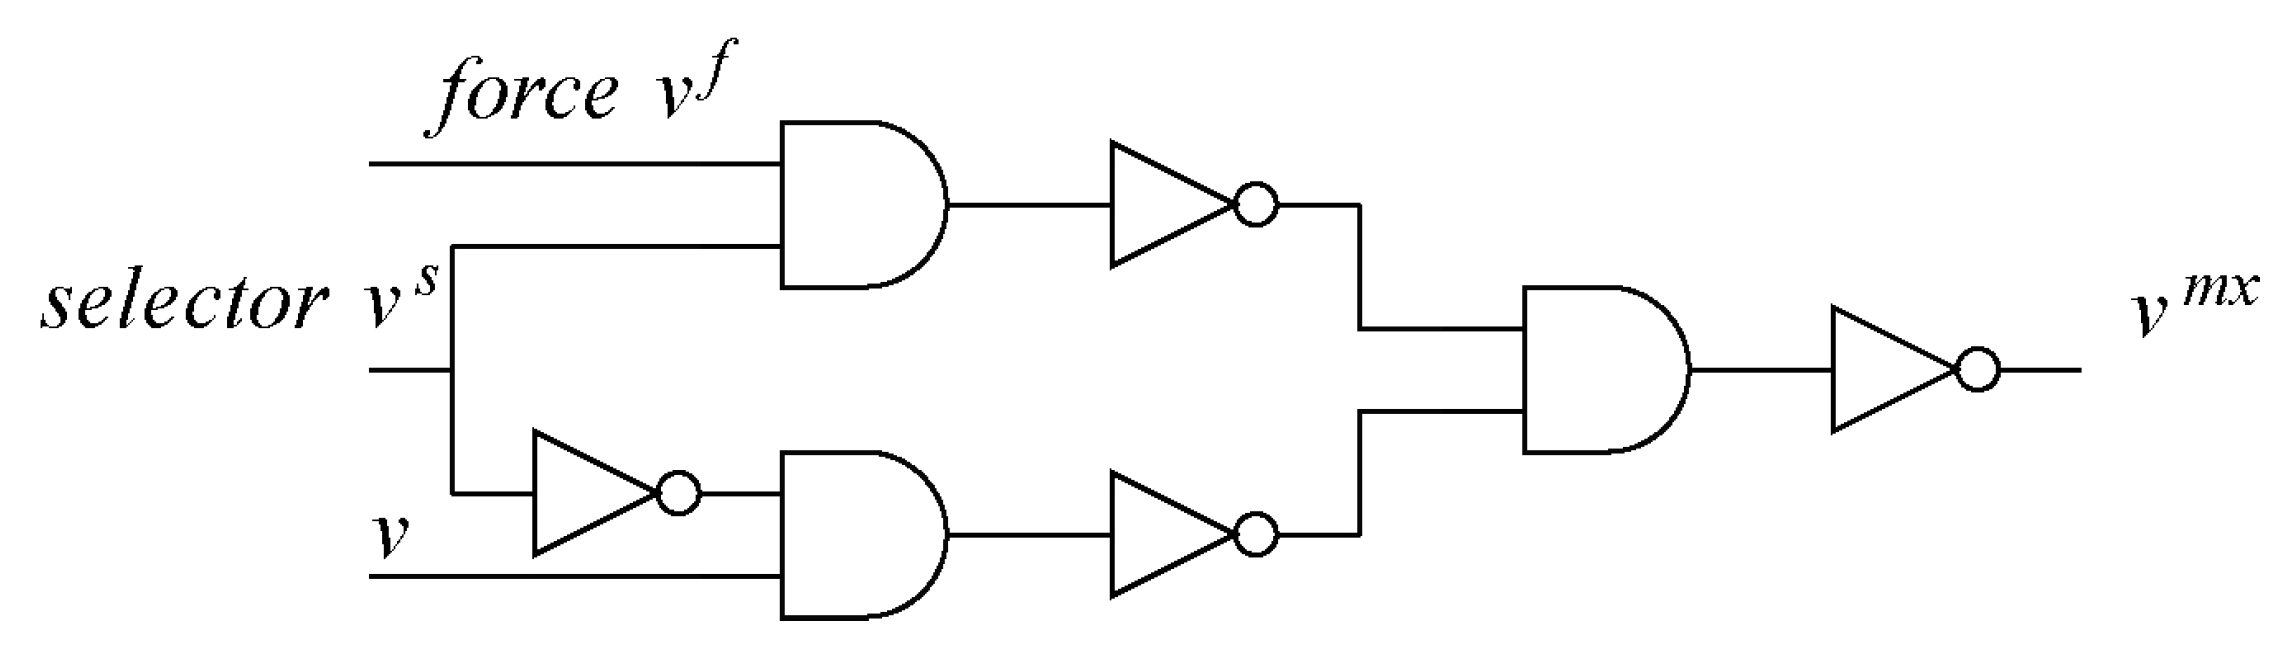
\includegraphics[width=0.37\textwidth]{figs/screenshot_multiplexer.png}
%  \vspace{-0.1in}
%  \caption{Multiplexer for introducing mutations into circuits}\label{fig:multiplexer}
%\end{figure}
%
%
%To introduce mutations, a multiplexer is introduced into the graph for the mutated vertex $v$ as shown in Figure~\ref{fig:multiplexer}, and all edges connected to $v$ are connected to $v^{mx}$.   If the selector signal $v^{s}$ is true, then the mutated signal $v^{f}$ is emitted instead of the original signal $v$.  To model stuck-at faults, $v^{f}$ is set to constant true or false, and to model non-deterministic faults, a ``fresh'' input signal is added to the model.
%\fi
%Of particular interest is the mutation that replaces a computed variable ({\em signal} in hardware) with a ``fresh'' input; this mutation is called a {\em nondeterminism mutation} with a coverage metric called (\nondetcov)~\cite{chockler2010coverage} and is discussed .
%s
%We can re-formalize their appr

%A net-list can immediately be mapped a transition system consisting of a conjunction of equations, where each vertex $v_i \in V_N$ is represented by a variable $u_i \in U$ in the transition system, and each non-input vertex is assigned by an equation based on its type and input edges.  So, for example, if you have a graph where three input vertices $(v_a, v_b, v_c)$ are connected by edges into a vertex $v_k$  that is an AND gate, it would become the equation: $u_k = u_a and u_b and u_c$.
%In the net-list structure, to mutate a vertex $v_i$, authors in \cite{chockler2010coverage} describes the technique of adding a  multiplexer to $N$. Then, the  edges  of  the  net-list are modified such  that  the  tails  of  all  the edges directed from
%$v_i$ are changed to the output of the multiplexer, which replaces
%$E_N$ with a new set of edges $E_M$ in the mutated net-list.
%Accordingly, the transition system of a mutated design can be constructed w.r.t $E_M$. That is to say, the mutated transition relation would have one additional top-level conjunction
%and be also structured based upon the new signal connections obtained by $E_M$.
% Given this representation, we can define nondeterministic coverage as follows:
%

%Using  $\nondetcov$, the coverage score of specification $P$ is computed by
%\[
%   \frac{ | \nondetcov (P)|}{|T|}
%\]
%
%\noindent It is straightforward to define stuck-at-true and stuck-at-false coverage by replacing \inputnode\ by constant 1 or 0, respectively.





